%!TEX TS-program = xelatex
%!TEX encoding = UTF-8 Unicode
\documentclass[12pt, xcolor=dvipsnames]{beamer}
\definecolor{slight}{gray}{0.9}
\fboxsep=10pt
\usecolortheme[named=Royal Blue]{structure}
\useinnertheme{circles}
\usepackage[no-math]{fontspec}
\usepackage{xltxtra, xunicode}
\usepackage[utf8]{inputenc}
%\usepackage[sc, osf]{mathpazo}
\usepackage[minionint, lf, mathtabular]{MinionPro}
\setmainfont[Mapping=tex-text]{Minion Web Pro}
\setsansfont[Mapping=tex-text]{Myriad Web Pro}
\setmonofont[Scale=MatchLowercase]{Source Code Pro}
\usefonttheme{professionalfonts}
%% 中文字配置
\usepackage[
CJKmath=true, indentfirst=false, PunctStyle={quanjiao},
CheckSingle=true, SlantFont, BoldFont
]{xeCJK}
\setCJKmainfont[Scale=0.9, BoldFont=Hiragino Mincho ProN W6]{Hiragino Mincho ProN W3}
\setCJKsansfont[Scale=0.9, BoldFont=Hiragino Sans W6]{Hiragino Sans W4}
%\setCJKsansfont[Scale=0.9, BoldFont=Hiragino Sans CNS W6]{Hiragino Sans CNS W3}
%\setCJKsansfont[Scale=0.9, BoldFont=Hiragino Sans W7]{Hiragino Sans W4}
%\setCJKsansfont[Scale=0.9, BoldFont=Source Han Sans UI TC Bold]{Source Han Sans UI TC Regular}
%\setCJKsansfont[Scale=0.9, BoldFont=PingFang TC Semibold]{PingFang TC Regular}
\setCJKmonofont[Scale=0.9, BoldFont=Yuanti TC Regular]{Hiragino Maru Gothic ProN W4}
\usepackage{fancyvrb, attachfile2, pstricks}
\usepackage{graphicx}
\setbeamerfont{page number in head/foot}{size=\tiny}
\setbeamertemplate{footline}[frame number]
\usepackage{xmpmulti, booktabs, multicol}
\setbeamertemplate{navigation symbols}{}
\let\WriteBookmarks\relax
\usepackage{dcolumn}
\newcolumntype{.}[1]{D{.}{.}{#1}}
\newcolumntype{,}[1]{D{,}{,}{#1}}

\linespread{1.25}

\setbeamersize{text margin left=.8em, text margin right=.6em}

\makeatletter
\defbeamertemplate{itemize item}{mycircle}{\LARGE\raise-1.6pt\hbox{\textbullet}}
\makeatother

\setbeamertemplate{itemize item}[mycircle]
\setbeamertemplate{itemize subitem}[triangle]
\setlength\leftmargini{1.3em}
\setlength\leftmarginii{1em}


%\CTXFR
\title{\bf{\Huge {}\\[-2mm] Principles of Economics \\[2mm] Review Session}}
\author{{\Large 張耕齊\\[2mm] Keng-Chi Chang}}
\institute{{}\\[-7mm]\footnotesize\tt{<r03323070@ntu.edu.tw>}\\[2mm]}
\date{\large 2016.10.05}
\begin{document}
\fontsize{12}{14pt}\selectfont


\begin{frame}
\titlepage
\end{frame}


\begin{frame}
\frametitle{\bf About Me \& Wednesday's Session}
\begin{itemize}
\item Econ B00, Exchange in UW-Madison, Econ Master-ing
\item Small TA, usually doesn't teach
\item Office Hour: Thursday 14:20-15:10 Social Science 650
\begin{itemize}
\item Don't just come for answers, show your work
\end{itemize}
\item Review important concepts and go through some HW
\item Interrupt me when you cannot understand or I made mistakes
\item Reserve some time for other questions
\begin{itemize}
\item Questions I supplied may different from your need
\item Questions differ but concepts are similar
\end{itemize}
\item Let me know if you have any suggestions
\end{itemize}
\end{frame}


\begin{frame}
\frametitle{\bf Chapter 3 in a Nutshell}
\begin{itemize}
\item Net benefit is maximized when marginal benefit = marginal cost
\item Why does this matter? 
\begin{itemize}
\item Sometimes we don't know what net benefit really means
\item But we can still make decisions using marginal information
\item Marginal analysis also reduces calculations
\item See ALL 3-4, ALL 3-7
\end{itemize}
\end{itemize}
\end{frame}

\begin{frame}
\frametitle{\bf Marginal Analysis}
\small \textsf{\bfseries ALL 3-8.} Assume that your country’s income tax structure has the following tax rates: if your income is \$30,000 or less you pay no income tax; if your income is above \$30,000, you pay 30 percent of the amount above \$30,000. 

You have three alternatives. You could not work at all, you could work half time, or you could work full time. If you do not work at all, you will earn \$0; if you work half-time you will earn \$30,000; and if you work full-time, you will earn \$60,000. Any time you do not work, you can spend surfing. You love to surf: surfing full-time is worth \$50,000 per year to you, surfing half time is worth \$25,000 per year to you, and not surfing at all is worth nothing to you. As you are making your decision about how much to work, should you pay attention to your average tax rate or to your marginal tax rate? Explain your answer carefully.
\end{frame}



\begin{frame}
\frametitle{\bf Chapter 4 in a Nutshell}
\begin{itemize}
\item Price and quantity demanded depicts the demand curve
\item Law of Demand: $\Delta Q_X^d/ \Delta P_X<0$
\item Factors other than the above two shifts the demand curve
\begin{itemize}
\item This means quantity demanded changes at any given price
\item Price of related goods $Y$
\item If $\Delta Q_X^d/ \Delta P_Y>0$ we call $Y$ a substitute 替代品 of $X$
\item If $\Delta Q_X^d/ \Delta P_Y<0$ we call $Y$ a complement 互補品 of $X$
\item Your income $I$
\item If $\Delta Q_X^d/ \Delta I>0$ we call $X$ a normal good 正常財
\item If $\Delta Q_X^d/ \Delta I<0$ we call $X$ an inferior good 劣等財
\item Expectations, tastes, number of buyers, ...
\end{itemize}
\item Similar for the supply side
\end{itemize}
\end{frame}



\begin{frame}
\frametitle{\bf Chapter 4 in a Nutshell}
\begin{itemize}
\item Market demand/supply is the sum of individual quantity demanded/supplied for some given price
\[Q_X^d(P_X)=Q_{1,X}^d(P_X)+\cdots+Q_{n,X}^d(P_X)=\sum^n_{i=1}Q_{i,X}^d(P_X)\]\\[-5mm]
\[Q_X^s(P_X)=Q_{1,X}^s(P_X)+\cdots+Q_{n,X}^s(P_X)=\sum^n_{i=1}Q_{i,X}^s(P_X)\]
\item Achieve equilibrium if some price enables market demand equals market supply: $Q_X^d(P^*_X)=Q_X^s(P^*_X)$
\begin{itemize}
\item For $P_X<P^*_X$: Excess demand increases $P_X$
\item For $P_X>P^*_X$: Excess supply decreases $P_X$
\end{itemize}
\end{itemize}
\end{frame}


\begin{frame}
\frametitle{\bf Binding Price Floor}
\small \textsf{\bfseries ALL 4-10.} The UK government is contemplating introducing a minimum price for alcohol to reduce binge drinking and the consumption of alcohol in general. Suppose the following diagram shows the alcohol market in the UK. The current price of alcohol is 23 pence per unit, and 8 units of alcohol are consumed each week. What happens in the market if the government sets a minimum price of 30 pence per unit of alcohol? Will there be an excess supply or an excess demand for alcohol if the government adopts this policy? Explain.\end{frame}


\begin{frame}
\frametitle{\bf Binding Price Floor}
\small \textsf{\bfseries ALL 4-10.}
\begin{center}
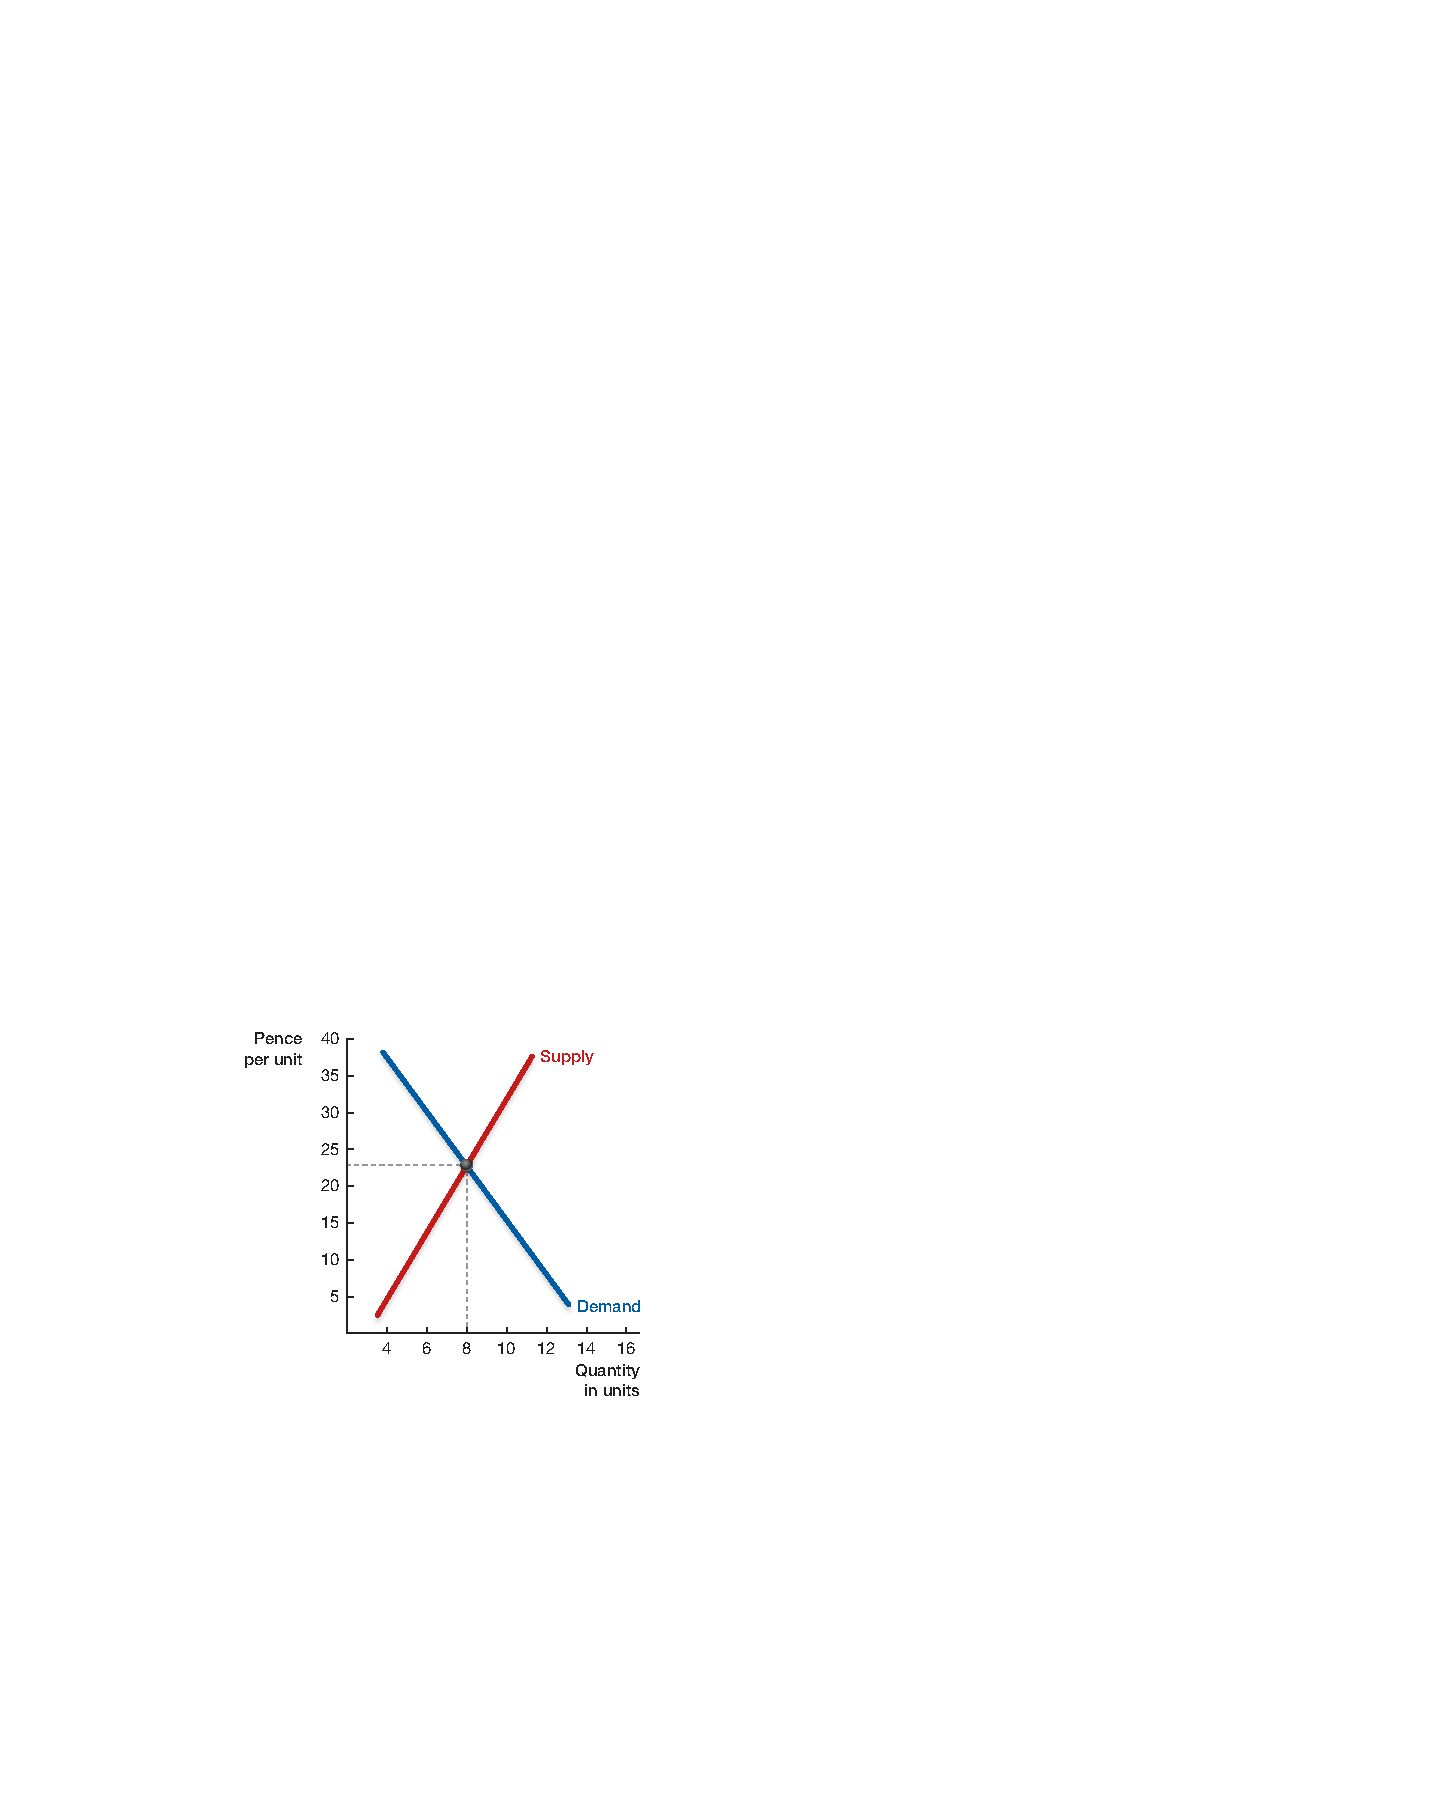
\includegraphics[width=.5\linewidth]{figures/4-10.pdf}
\end{center}
\vspace{-7mm}
Extension: Minimum wage (Midterm 2010 True or False Q7)\\
Price ceilings (Midterm 2009 Essay D1-D6, Midterm 2010 True or False Q6)
\end{frame}



\begin{frame}
\frametitle{\bf Expectations}
\small \textsf{\bfseries Midterm 2008 Essay Part A.} 
\begin{enumerate}\itemsep-0.5ex
\item [1.] Do you expect vegetable prices to increase or decrease after a typhoon? Why?
\item [2.]  Is the price change due to a demand shift or supply shift, or both? To which direction(s)?
\item [3.]  Why would one want to jump the gun and buy more vegetables before a typhoon?
\item [4.]  If more people are jumping the gun, how would vegetable prices change before a
typhoon? Explain.
\item [5.]  Why would farmers want to jump the gun and harvest more vegetables before a
typhoon?
\item [6.]  If more farmers jump the gun, how would vegetable prices change before a typhoon?
Explain.
\end{enumerate}
\end{frame}


\begin{frame}
\frametitle{\bf Expectations}
\small \textsf{\bfseries Midterm 2008 Essay Part A.} 
\begin{enumerate}\itemsep-0.5ex
\item [7.]  According to the article above, how did the equilibrium price and quantity of the
vegetable market change before a typhoon?
\item [8.]  Plot the demand and supply shifts for the vegetable market before a typhoon. Indicate
which shift is larger (according to your answers to the previous question).
\item [9.]  According to the last paragraph, some vegetables had smaller price hikes than others.
Why do you think this would be possible?
\end{enumerate}
\end{frame}


\end{document}